%%%%%%%%%%%%%%%%%%%%%%%%%%%%%%%%%%%%%%%%%%%%%%%%%%%%%%%%%%%%%%%%%%%%%%%%%%%%%%%%%
%%%
%%%%%%%%%%%%%%%%%%%%%%%%%%%%%%%%%%%%%%%%%%%%%%%%%%%%%%%%%%%%%%%%%%%%%%%%%%%%%%%%%
\section{BERT}
Multiple attempts were made to a develop a BERT \cite{devlin_bert} based classification model, two of the three attempts were failures, however the final 
model achieved near state of the art performance on the test dataset. 

\subsection{Attempt One}
The initial attempt at training BERT was performed on a complex model. The model was passed through multiple 


\subsection{Attempt Two}


\subsection{Attempt Three}

\subsubsection{Determinging token length}
In BERT , there is a max token length of the pretrained models of 512 tokens. This obviously presents a challenge for us, especially considering that some 
of the space available needs to be used for the special tokens. There are solutions to this problem such as Longformer and Big Bird which are designed for large documents, 
but they introduce more training time. 

In order to determine if Big Bird or Longformer should be used, a simple visualisation was used \todo{use synonym} to asses the amount of entries that 
fit under the BERT imposed limit of 512 tokens. 

\begin{figure}[ht]
  \centering
  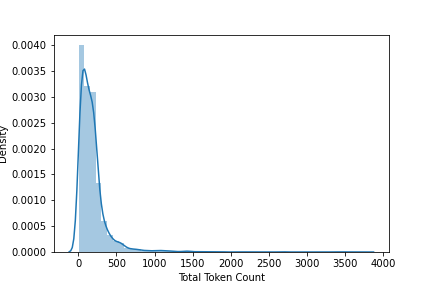
\includegraphics[width=\columnwidth]{total_length_dist}
  \caption{Distribution plot of combined token lengths}
  \label{fig:tdist}
\end{figure}

As seen from \cref{fig:tdist}, the token length can be capped at 512 and we should still preserve the discourse captured in the set of tweets.
However, in order to maximise the information used by the BERT model, stopwords were removed as well. 

\subsubsection{Model}
The model was developed using PyTorch \cite{pytorch} and trained via a TPU instance on Google Colab first. 
The Google Colab based training failed to train after a certain amount of time, this was due to the fact that Google Colab times out 
sessions after a small period (relative to the training time) of time. In order to combat this
